% Activate the following line by filling in the right side. If for example the name of the root file is Main.tex, write
% "...root = Main.tex" if the chapter file is in the same directory, and "...root = ../Main.tex" if the chapter is in a subdirectory.
 
%!TEX root =  dissertation.tex

\chapter[Analysis]{Analysis}

\section{Usability result and analysis}

In evaluating HemeWeb's usability and capability to run and reproduce simulation, I conducted a usability evaluation via an online survey hosted by Google Form\footnote{\url{https://goo.gl/forms/toYsRwnGIGumMBUD2}}. Respondents are given 2 tasks to complete, which are to run a simulation and reproduce past simulation. After the tasks, they are given statements to respond to. Based on the answers, I analyze respondent's answers with regards to HemeWeb's usability.


\subsection{Demography}


\vspace{0.5cm}

\noindent%
\begin{minipage}{\linewidth}% to keep image and caption on one page
\makebox[\linewidth]{
  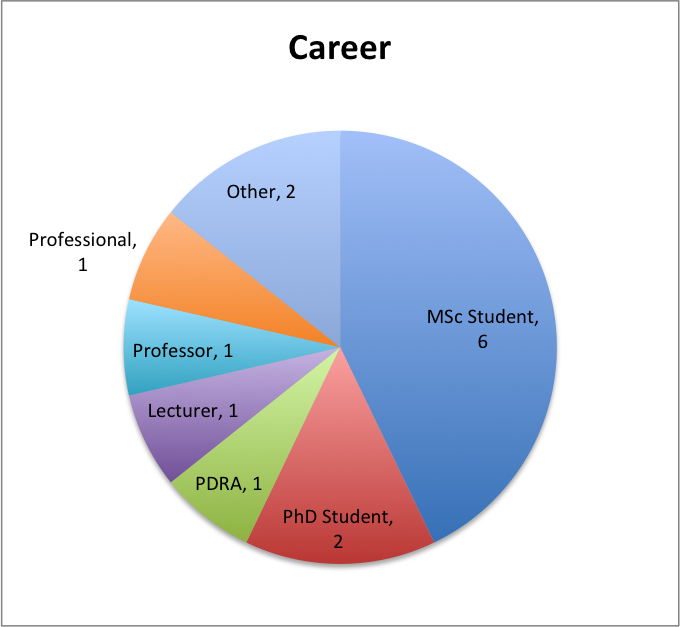
\includegraphics[keepaspectratio=true,scale=0.7]{../resources/evaluation/usability/career.png}
 }
\captionof{figure}{Career stage distribution} \label{fig:survey-career}%      only if needed  
\end{minipage}

\vspace{0.5cm}

\vspace{0.5cm}

\noindent%
\begin{minipage}{\linewidth}% to keep image and caption on one page
\makebox[\linewidth]{
  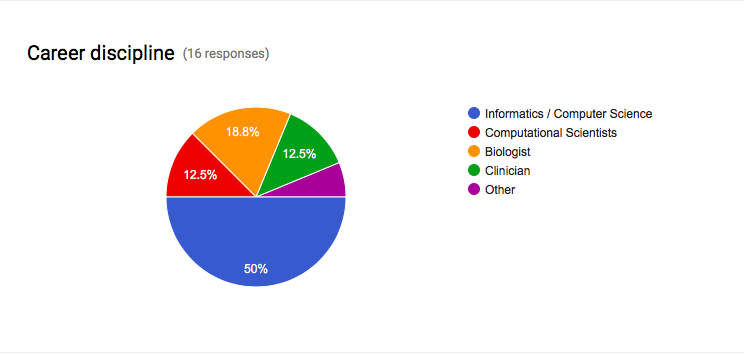
\includegraphics[keepaspectratio=true,scale=0.8]{../resources/evaluation/usability/discipline.png}
 }
\captionof{figure}{Career discipline} \label{fig:survey-discipline}%      only if needed  
\end{minipage}

\vspace{0.5cm}


The survey was filled by 16 respondents over the period of 10 days (3rd August 2016 - 10th August 2016)\footnote{Raw and compiled responses can be found at \url{https://github.com/SeiryuZ/HemeWeb/tree/master/documents/resources/evaluation/usability} \label{footnote:response}}. From all the responses, one of the respondent were unable to run both of the tasks, citing errors preventing him to run the scenarios which we cannot reproduce. Due to this problem, we have to remove this particular response from our analysis because it will not add meaningful information about the usability of the system when the scenarios are not run. In total, we got 15 valid responses out of the questionnaire period.

Figure \ref{fig:survey-career} and \ref{fig:survey-discipline} illustrates the distribution of career stage and discipline of our participants. Based on this distribution, we can further analyze the response we get on the survey questions based on their background. One meaningful comparison we can make is when we classify respondents based on their informatics-related discipline. 10 of our respondents, or 2 out of 3, are related to informatics background, while 5 of the respondents can be considered as domain experts which consists of Biologist, Clinician, and Biophysicist.


\vspace{0.5cm}

\noindent%
\begin{minipage}{\linewidth}% to keep image and caption on one page
\makebox[\linewidth]{
  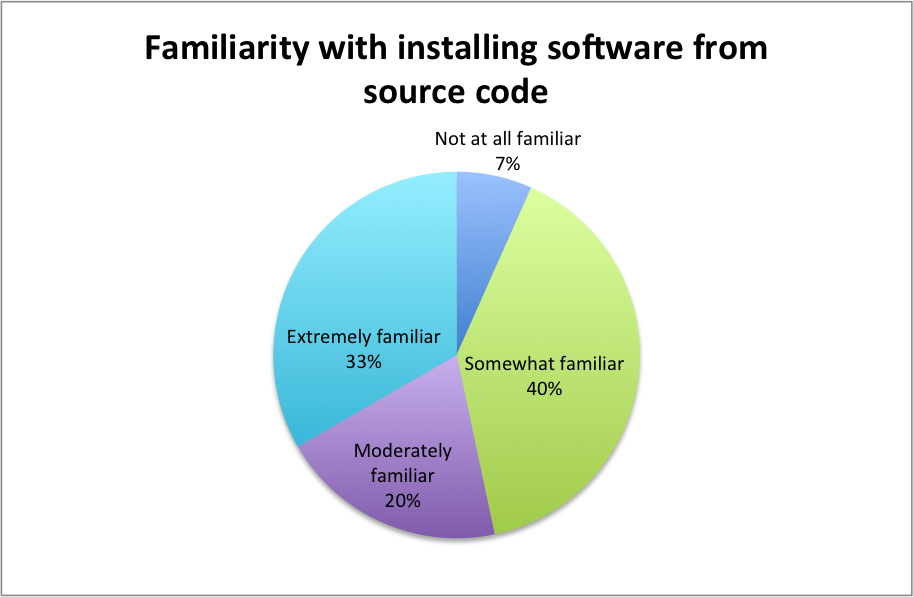
\includegraphics[keepaspectratio=true,scale=0.8]{../resources/evaluation/usability/source_code.png}
 }
\captionof{figure}{Familiarity with installing software from source code} \label{fig:survey-source}%      only if needed  
\end{minipage}

\vspace{0.5cm}

\noindent%
\begin{minipage}{\linewidth}% to keep image and caption on one page
\makebox[\linewidth]{
  
\includegraphics[keepaspectratio=true,scale=0.8]{../resources/evaluation/usability/browser.png}
 }
\captionof{figure}{Familiarity with web browser} \label{fig:survey-browser}%      only if needed  
\end{minipage}

\vspace{0.5cm}

\noindent%
\begin{minipage}{\linewidth}% to keep image and caption on one page
\makebox[\linewidth]{
  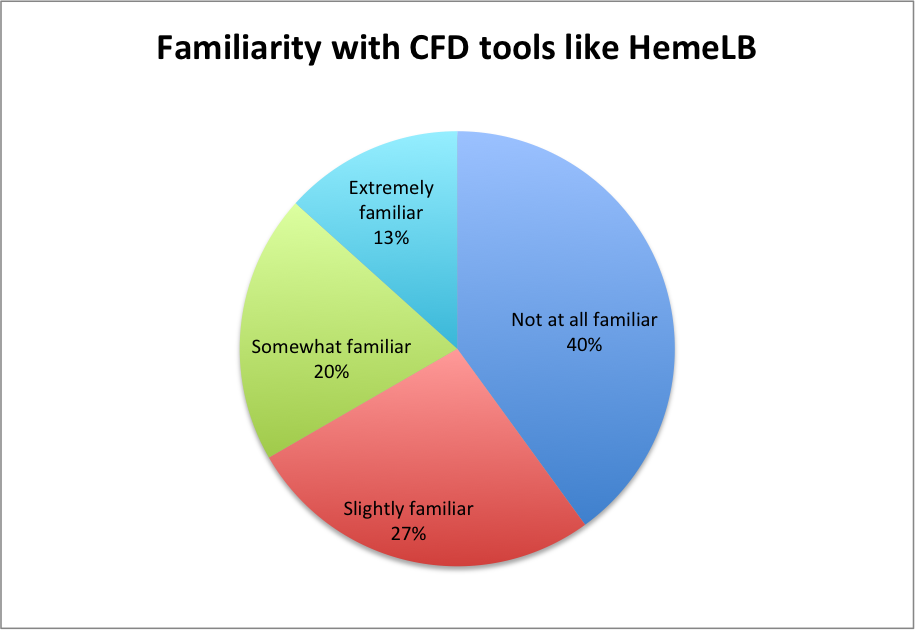
\includegraphics[keepaspectratio=true,scale=0.8]{../resources/evaluation/usability/hemelb.png}
 }
\captionof{figure}{Familiarity with CFD tools like HemeLB} \label{fig:survey-hemelb}%      only if needed  
\end{minipage}

\vspace{0.5cm}


We can also further classify analyze the respondents' response based on the familiarity with browsers, computational fluid dynamic tools, and installing software from source code. All of this are shown in Figure \ref{fig:survey-source}, \ref{fig:survey-browser}, and \ref{fig:survey-hemelb}.



\subsection{Scenario 1: Run a HemeLB simulation}

In this scenario, respondents are provided with two input files necessary for running a simulation. Respondents are asked to download the files beforehand and follow the instructions provided in the online questionnaire to run a HemeLB simulation using HemeWeb.  After running the simulation, Respondents are then asked to state agreement with three positive statements about HemeWeb that will measure their satisfaction with HemeWeb in running a HemeLB simulation scenario. 



\vspace{0.5cm}

\noindent%
\begin{minipage}{\linewidth}% to keep image and caption on one page
\makebox[\linewidth]{
  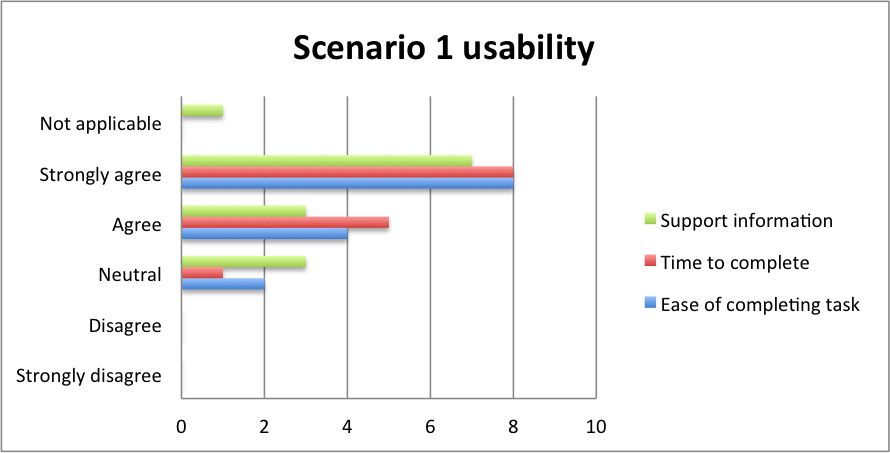
\includegraphics[keepaspectratio=true,scale=0.9]{../resources/evaluation/usability/scenario1_usability.png}
 }
\captionof{figure}{Scenario 1 usability} \label{fig:survey-s1-usability}%      only if needed  
\end{minipage}
\vspace{0.5cm}


Figure \ref{fig:survey-s1-usability} show the responses for the three positive statements about HemeWeb. From the 15 valid responses we get, all of them did not skip the instructions to run the simulation. From the responses, respondents tend to agree that they are satisfied with HemeWeb in running a HemeLB simulation. Respondents tend to equally agree on the three positive statements about the ease of completing a task, time to complete, and supporting information available to help complete the task. However, one respondent fills out "Not Applicable" towards the statement about HemeWeb giving them enough support information. This could mean that the scenario undertook to give enough information to agree or disagree with the statements.

In addition to the general sentiment of the respondents, we can also put a number value to the responses to further measure the satisfaction objectively. We can calculate the After Scenario Questionnaire(ASQ) score. To do this, we assign an integer value for each response; 1 for "Strongly disagree", 2 for "Disagree", 3 for "Neutral", 4 for "Agree", and 5 for "Strongly agree". With this value, we can take the mean of the response for each question as a single ASQ score for the respondent. If a respondent skips a question, we can take the average of the remaining responses as the score. With this mechanism, we can determine the respondent's average ASQ score, which is 4.36. This score falls between "Agree" and "Strongly agree", therefore, we can conclude that in general respondents tend to agree that they are satisfied with HemeWeb with regards to running a HemeLB simulation.



%Our hypothesis is that users will generally find using web interface is usable and the data seemed to support that. It is much easier for user to complete a task when using point and click interface rather than requiring them to recall commands to do the tasks, especially when they are not familiar with the tools.
%
%
%Next, respondents are given a high overview of replicating the tasks done in HemeWeb but using command line interface. Respondents are not asked to run the scenario in their command line interface because we cannot make sure the necessary tools are installed on respondent's computer.

\vspace{0.5cm}

\noindent%
\begin{minipage}{\linewidth}% to keep image and caption on one page
\makebox[\linewidth]{
  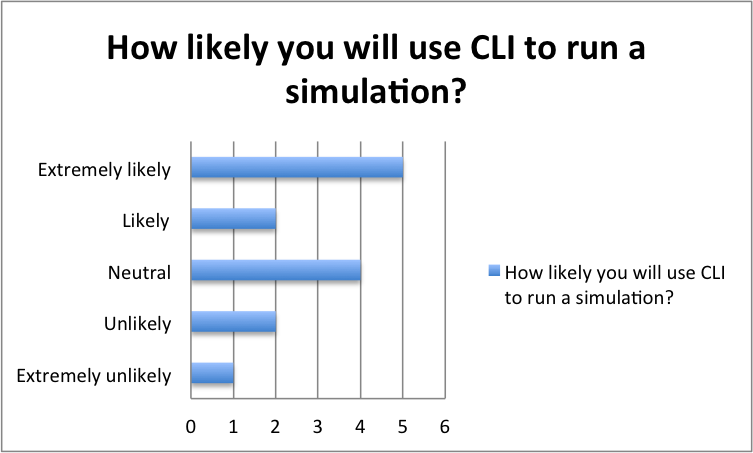
\includegraphics[keepaspectratio=true,scale=0.9]{../resources/evaluation/usability/scenario1_cli.png}
 }
\captionof{figure}{Scenario 1 command line preference} \label{fig:survey-s1-cli}%      only if needed  
\end{minipage}

\vspace{0.5cm}

\noindent%
\begin{minipage}{\linewidth}% to keep image and caption on one page
\makebox[\linewidth]{
  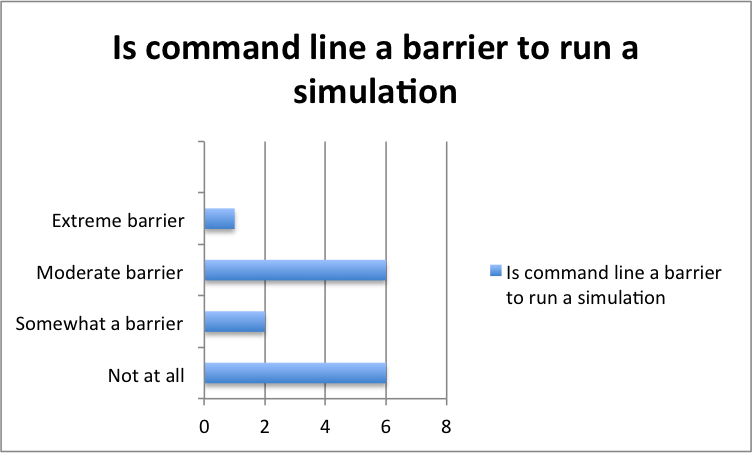
\includegraphics[keepaspectratio=true,scale=0.9]{../resources/evaluation/usability/scenario1_cli_barrier.png}
 }
\captionof{figure}{Scenario 1 barrier in using command line} \label{fig:survey-s1-cli-barrier}%      only if needed  
\end{minipage}

\vspace{0.5cm}

After the above sentiments about using HemeWeb to run a HemeLB simulation, respondents were asked about their sentiment about using command line interface(CLI) to do the same activity. Figure \ref{fig:survey-s1-cli} and \ref{fig:survey-s1-cli-barrier} shows the respondent's inclination in using CLI. Respondents are generally open to the likelihood of them running a simulation using CLI. If we quantify the results like we did with the ASQ score, we get 3.46, which is somewhere between neutral and likely. 

The distribution of the responses also is quite spread out, that respondents fill out all possible responses with   the highest frequency being "Extremely Likely" with 5 responses. However, we have to keep it mind the general background of the respondents that may explain the highest frequency answer being "Extremely Likely", which is about familiarity with installing software with source code. To build software with source code, one will interact with the command line interface quite often. 14 of our respondents answered at least somewhat familiar with building software from source code, that can explain that our respondents are mostly quite competent in operating command line interface and would not shy away in using the command line interface. In addition to that, 2 out of 3 respondents has backgrounds in informatics and computational science. This could in effect explains why the respondents feel they are likely and extremely likely to do the same in CLI. 

However, not all respondents who are at least somewhat familiar with building software from source code skew towards to the likely side of using CLI. There are respondents that, while familiar with the interface, running a HemeLB simulation using CLI is unlikely to be done by them. These responses might be explained by respondents' sentiment in using command line interface. This is further supported by the response of CLI being a barrier for the respondents. While 6 of the respondents think it is not a barrier at all to use CLI, 9 of the respondents answered at least it is somewhat a barrier. With 6 of the 9 respondents, feel it is a moderate barrier, and 1 of the 9 feel it as an Extreme barrier. From these results, we can safely say that using command line interface is a form of a barrier to run HemeLB for almost two-third of the respondents.





\subsection{Scenario 2: Reproduce past simulation}

In the second scenario, respondents are asked to reproduce past simulation with HemeWeb. They are given instructions in the online questionnaire to create a HemeLB simulation job from past simulation. They have to enter a URL that contains past simulation job and modifies the simulation parameters to avoid only replicating the past simulation without changes. After reproducing past simulation, respondents are then asked to state agreement with the same questions like they had in the first scenario. These questions will also measure their satisfaction with HemeLB in reproducing past simulation.


\vspace{0.5cm}

\noindent%
\begin{minipage}{\linewidth}% to keep image and caption on one page
\makebox[\linewidth]{
  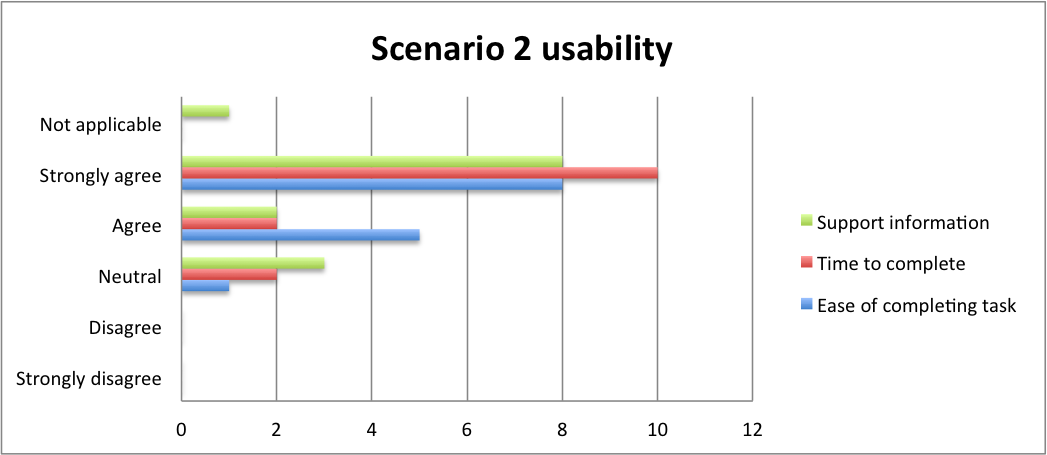
\includegraphics[keepaspectratio=true,scale=0.9]{../resources/evaluation/usability/scenario2_usability.png}
 }
\captionof{figure}{Scenario 2 usability} \label{fig:survey-s2-usability}%      only if needed  
\end{minipage}
\vspace{0.5cm}

Figure \ref{fig:survey-s2-usability} shows the general sentiment to the three statements that we provided. Generally, the response tends to skew towards agreeing that respondents are satisfied with HemeWeb with regards to reproducing past simulation. However, it has to be noted that 1 of the respondent skipped the instructions. This particular respondent did not give out any comments about encountering any problems, so we cannot deduce whether his skipping the instruction is due to usability problems or he just wants to skip it. Without further information, we cannot deduce why he skips the instructions.

Also, similar to the first scenario, one respondent fills out "Not Applicable" to support information statement. Once again, this could mean that the scenario does not provide the respondent with enough information to fill out their agreement to the statement. In a nutshell, respondents tend to agree that HemeWeb is satisfying to use for the purpose of reproducing past simulation. If we convert the responses to a numerical value, we will get 4.31 of ASQ score. Which is in line with the sentiment that I described. The ASQ score falls between agreeing and strongly agree towards the positive statements we provided.


\vspace{0.5cm}

\noindent%
\begin{minipage}{\linewidth}% to keep image and caption on one page
\makebox[\linewidth]{
  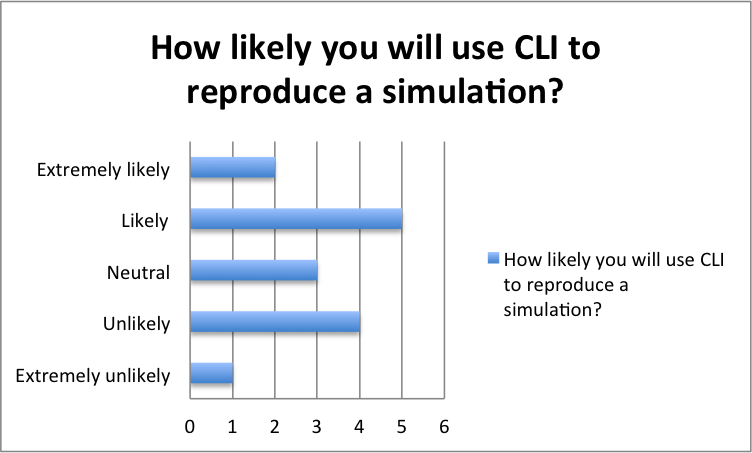
\includegraphics[keepaspectratio=true,scale=0.9]{../resources/evaluation/usability/scenario2_cli.png}
 }
\captionof{figure}{Scenario 2 command line preference} \label{fig:survey-s2-cli}%      only if needed  
\end{minipage}

\vspace{0.5cm}

\noindent%
\begin{minipage}{\linewidth}% to keep image and caption on one page
\makebox[\linewidth]{
  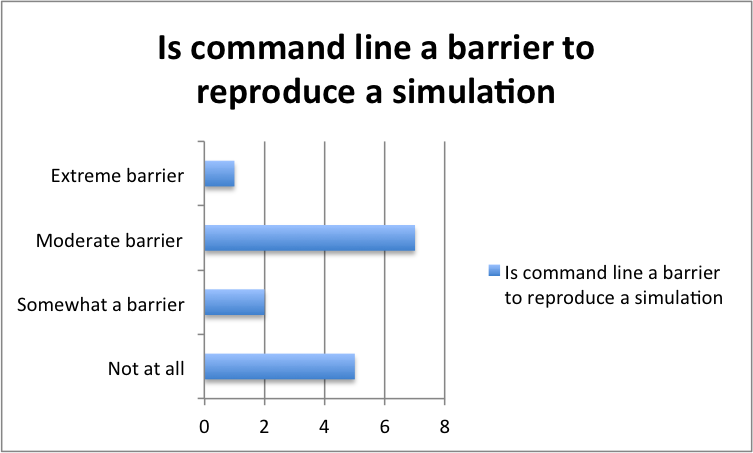
\includegraphics[keepaspectratio=true,scale=0.9]{../resources/evaluation/usability/scenario2_cli_barrier.png}
 }
\captionof{figure}{Scenario 2 barrier in using command line} \label{fig:survey-s2-cli-barrier}%      only if needed  
\end{minipage}

\vspace{0.5cm}

Respondents are then given high-level steps to reproduce past simulation using the command line interface.  Figure \ref{fig:survey-s2-cli} and \ref{fig:survey-s2-cli-barrier} shows the respondent's response. Similar to the first scenario, the respondents are generally open to the idea of operating command line interface to do their tasks. However, the scenario to reproduce past simulation provides a bit difference in the distribution of the answers. While in the first scenario the highest frequency of the answer is "Extremely likely", the highest one in this scenario is "Likely". 

This change of the highest frequency might be because there are extra step which might complicate the scenario to reproduce past simulation. respondents are more hesitant to answer "Extremely likely". However, the general nuance of the answer is still the same, respondents are generally not afraid of using command line interface to do this task. If we convert the answers into a numerical form like we did before, we got 3.2, which is between neutral and likely. 

In addition, same observation as the first scenario can be made. While some respondents are likely to reproduce past simulations, there are those who are not likely to reproduce past simulations even with their background that have dealt with building software from source code. This can be explained by Figure \ref{fig:survey-s2-cli-barrier} where only 5 of the respondents did not feel that using CLI is a barrier at all. 2 of the respondents feel using CLI is somewhat a barrier, 7 feel it as a moderate barrier, and  1 feels it as an extreme barrier. This means that this 10 respondent agree that CLI is a form of barrier to them, however small.


\subsection{Overall usability}


Here, I will discuss the overall usability of the system using the Post Study System Usability Questionnaire(PSSUQ) as the basis. This part of the questionnaire consists of 19 questions that can be divided into measuring three different component of the systems. These are system usefulness, information quality, and the interface quality. I will discuss each of them in details.

%%%%%%%%%%%%%%%%%%%%%%%%%%%%%%%%%%%
%  SYSTEM USEFULNESS 
%%%%%%%%%%%%%%%%%%%%%%%%%%%%%%%%%%%
\begin{center}
\captionof{table}{System usefulness}\label{table:overall-usability}
\scalebox{0.75}{

\begin{tabular}{|l|c|c|c|c|c|c|}
\hline
                                                                                                         & \multicolumn{1}{l|}{\begin{tabular}[c]{@{}l@{}}Strongly\\ disagree\end{tabular}} & \multicolumn{1}{l|}{Disagree} & \multicolumn{1}{l|}{Neutral} & \multicolumn{1}{l|}{Agree} & \multicolumn{1}{l|}{\begin{tabular}[c]{@{}l@{}}Strongly\\ agree\end{tabular}} & \multicolumn{1}{l|}{\begin{tabular}[c]{@{}l@{}}Not\\ applicable\end{tabular}} \\ \hline
\begin{tabular}[c]{@{}l@{}}Overall, I am satisfied with how easy it is\\ to use this system\end{tabular} & 0                                                                                & 0                             & 0                            & 8                          & 7                                                                             & 0                                                                             \\ \hline
It was simple to use this system                                                                         & 0                                                                                & 0                             & 0                            & 2                          & 13                                                                            & 0                                                                             \\ \hline
\begin{tabular}[c]{@{}l@{}}I can effectively complete my work\\ using this system\end{tabular}           & 1                                                                                & 1                             & 2                            & 3                          & 4                                                                             & 4                                                                             \\ \hline
\begin{tabular}[c]{@{}l@{}}I am able to complete my work quickly\\ using this system\end{tabular}        & 0                                                                                & 1                             & 3                            & 3                          & 6                                                                             & 2                                                                             \\ \hline
\begin{tabular}[c]{@{}l@{}}I am able to efficiently complete my work\\ using this system\end{tabular}    & 0                                                                                & 2                             & 2                            & 4                          & 5                                                                             & 2                                                                             \\ \hline
I feel comfortable using this system                                                                     & 1                                                                                & 1                             & 0                            & 3                          & 10                                                                            & 0                                                                             \\ \hline
It was easy to learn to use this system                                                                  & 0                                                                                & 0                             & 2                            & 0                          & 13                                                                            & 0                                                                             \\ \hline
\begin{tabular}[c]{@{}l@{}}I believe I became productive quickly\\ using this system\end{tabular}        & 0                                                                                & 1                             & 2                            & 3                          & 5                                                                             & 4                                                                             \\ \hline
\end{tabular}
}
\end{center}
\vspace{0.5cm}

Table \ref{table:overall-usability} shows the respondents sentiment towards positive statements about the system usefulness. Generally, we can see the distribution of respondents mostly agreeing with the statements presented. Ignoring the respondents that answered with "Not applicable", we can find the distribution is skewed to the agreeing side of the statements. There are respondents that disagree or even strongly disagree with some questions. However, the frequency is much lower compared towards the frequency of people agreeing to the statements. 

Converting  the response into a numerical value, we can get the score of 4.27 of system usefulness, which is quite high. However, there are still some improvements that can be made, and it is apparent in the feedbacks\footnote{See raw survey response - Footnote \ref{footnote:response}} of the system we got. In addition, there are respondents that respond to the statement by answering Not applicable. It is mostly on the framing of the simulation as a 'work'. Respondents might have no point of reference whether using the HemeLb via HemeWeb is quicker or efficiently because they are new to the system. This is apparent from their background that they don't  have familiarity with HemeLB.


%%%%%%%%%%%%%%%%%%%%%%%%%%%%%%%%%%%
%  INFO QUALITY
%%%%%%%%%%%%%%%%%%%%%%%%%%%%%%%%%%%

\begin{center}
\captionof{table}{Information quality}\label{table:overall-info-quality}
\scalebox{0.75}{
\begin{tabular}{|l|l|l|l|l|l|l|}
\hline
                                                                                                                                                                               & \begin{tabular}[c]{@{}l@{}}Strongly\\ disagree\end{tabular} & Disagree & Neutral & Agree & \begin{tabular}[c]{@{}l@{}}Strongly\\ agree\end{tabular} & \begin{tabular}[c]{@{}l@{}}Not\\ applicable\end{tabular} \\ \hline
\begin{tabular}[c]{@{}l@{}}The system gives error messages that\\  clearly tell me how to fix problems\end{tabular}                                                            & 0                                                           & 2        & 1       & 4     & 2                                                        & 6                                                        \\ \hline
\begin{tabular}[c]{@{}l@{}}Whenever I make a mistake using the system, \\ I recover easily and quickly\end{tabular}                                                            & 0                                                           & 0        & 5       & 1     & 3                                                        & 6                                                        \\ \hline
\begin{tabular}[c]{@{}l@{}}The information (such as online help, \\ on-screen messages, and other documentation)\\  provided with this system is clear\end{tabular}            & 0                                                           & 0        & 3       & 4     & 5                                                        & 3                                                        \\ \hline
It is easy to find the information I needed                                                                                                                                    & 0                                                           & 1        & 2       & 3     & 6                                                        & 3                                                        \\ \hline
\begin{tabular}[c]{@{}l@{}}The information (such as online help,\\  on-screen messages, and other documentation)\\  provided for the system is easy to understand\end{tabular} & 0                                                           & 1        & 2       & 5     & 6                                                        & 1                                                        \\ \hline
\begin{tabular}[c]{@{}l@{}}The information is effective in helping me\\  complete the tasks and scenarios\end{tabular}                                                         & 0                                                           & 1        & 4       & 2     & 7                                                        & 1                                                        \\ \hline
\begin{tabular}[c]{@{}l@{}}The organization of information on the \\ system screens is clear\end{tabular}                                                                      & 0                                                           & 0        & 3       & 8     & 4                                                        & 0                                                        \\ \hline
\end{tabular}

}
\end{center}
\vspace{0.5cm}

Table \ref{table:overall-info-quality} gives more insight on the respondents sentiment on HemeWeb's information quality. This includes information like error messages, documentation, the organization of this information, and etc. From seven positive statements that we presented. most respondents tend to agree that the information quality is good. The overall sentiment is more towards agreeing compared to disagreeing. If we convert the sentiment into a score, it will get 4.0 average score, Which falls under "Agree" sentiment.  

However, there are more respondents answering "Not applicable" in this part of the questionnaire. This led to the remaining answer having more contribution towards the average sentiment because many of the answers are not counted. For example, there are 6 ignored responses on the first statement about error messages. This is likely because the scenario given to the respondents will not give out an error message if they are correct the first time.  In the end, however, respondents tend to agree that information quality of HemeWeb is good.




%%%%%%%%%%%%%%%%%%%%%%%%%%%%%%%%%%%
%  INTERFACE QUALITY
%%%%%%%%%%%%%%%%%%%%%%%%%%%%%%%%%%%
\begin{center}
\captionof{table}{Interface quality}\label{table:overall-interface-quality}
\scalebox{0.75}{
\begin{tabular}{|l|l|l|l|l|l|l|}
\hline
                                                                                                                  & \begin{tabular}[c]{@{}l@{}}Strongly\\ disagree\end{tabular} & Disagree & Neutral & Agree & \begin{tabular}[c]{@{}l@{}}Strongly\\ agree\end{tabular} & \begin{tabular}[c]{@{}l@{}}Not\\ applicable\end{tabular} \\ \hline
The interface of this system is pleasant                                                                          & 1                                                           & 1        & 1       & 7     & 5                                                        & 0                                                        \\ \hline
I like using the interface of this system                                                                         & 0                                                           & 2        & 1       & 8     & 4                                                        & 0                                                        \\ \hline
\begin{tabular}[c]{@{}l@{}}This system has all the functions and\\  capabilities I expect it to have\end{tabular} & 1                                                           & 2        & 1       & 4     & 4                                                        & 3                                                        \\ \hline
\end{tabular}
}
\end{center}
\vspace{0.5cm}


Table \ref{table:overall-interface-quality} shows the respondents sentiment with regards to HemeWeb's interface quality. In it, we see respondents strongly disagree and disagree with positive statements about the interface. While in general, most respondents tend to agree that the interface is good, some disagree. When we see this particular response, it seemed that the respondent had trouble with the interface not rendering correctly in firefox. This feedback means that the browser compatibility of HemeWeb should be improved. There are parts of the interface which are broken if it is viewed on firefox. There are other respondents who dislike the XML editor based on their feedbacks. However, all this are subjective in nature and further testing of the interface is needed.

However, if we convert the respondents answer to a numerical value, we got 3.84, which is between neutral and agree. It shows that while some respondents find the interface quality is not up to their standards, some find it good enough although a lot can be improved. Browser compatibility, web form choice, user experience, and etc should be improved on the next iteration of HemeWeb.



\begin{center}
\captionof{table}{Overall user satisfaction quality}\label{table:overall-satisfaction}
\scalebox{0.75}{
\begin{tabular}{|l|l|l|l|l|l|l|}
\hline
                                         & \begin{tabular}[c]{@{}l@{}}Strongly\\ disagree\end{tabular} & Disagree               & Neutral                & Agree                  & \begin{tabular}[c]{@{}l@{}}Strongly\\ agree\end{tabular} & \begin{tabular}[c]{@{}l@{}}Not\\ applicable\end{tabular} \\ \hline
Overall, I am satisfied with this system & \multicolumn{1}{c|}{0}                                      & \multicolumn{1}{c|}{0} & \multicolumn{1}{c|}{2} & \multicolumn{1}{c|}{7} & \multicolumn{1}{c|}{6}                                   & \multicolumn{1}{c|}{0}                                   \\ \hline
\end{tabular}
}
\end{center}
\vspace{0.5cm}

The last part of the question is the overall perceived satisfaction that the user has in using the system. The distribution of the response can be found in Table \ref{table:overall-satisfaction}. Most of the respondents gravitate towards agreeing and strongly agreeing that they are satisfied with the system. When we convert it into a numerical mean, it is 4.26, which is between "Agree" and "Strongly agree". To get the overall user satisfaction score of the study, we average the numerical score between the 19 questions and we got 4.1. This means that the respondents mostly agree that they are satisfied with how the system performs,  inform, and looks like.

\section{Performance result and analysis}

In this section, I will discuss the performance benchmark of HemeLB simulation done in ARCHER supercomputer, INDY2 HPC cluster, and AWS EC2. Understanding the difference in performance is essential for HemeWeb project. In order to get the flexibility that the cloud vendors provide, we have to analyze what performance penalty we are incurring because of this design decision. 

In order to do this benchmark, we are going to rely on the report file that HemeLB produced. It is produced after each simulation is done and contains performance metric of each simulation like how many seconds are spent on communication, initializations, reading input files, and most importantly total simulation time. We are going to take a look at the total simulation time because it is the metric that captures the difference in the infrastructure better. We ran the simulation each time with the exact same configuration and input files. On each infrastructure, the simulations are done with an increasing number of compute node to measure the scaling of HemeLB.  From the produced output, then we can measure the performance difference between architecture.





\begin{center}

\captionof{table}{Performance comparison HemeLB on INDY2 vs AWS EC2}\label{table:perf}

\begin{tabular}{|c|c|c|}
\hline
\multicolumn{1}{|l|}{}            & \multicolumn{2}{c|}{Total simulation time in seconds}               \\ \hline
\multicolumn{1}{|c|}{\# of Cores (\# compute nodes)} & \multicolumn{1}{c|}{INDY2} & \multicolumn{1}{c|}{AWS EC2} \\ \hline
36 (1)                                & 24.7                       & 36.3                         \\ \hline
72 (2)                                & 12.7                       & 29.9                         \\ \hline
144 (3)                               & 7.08                       & 36.5                         \\ \hline
288 (4)                               & 3.44                       & 32.4                         \\ \hline
576 (5)                               & 1.81                       & 20.4                         \\ \hline
1152 (6)                              & 1.58                       & N/A                             \\ \hline
\end{tabular}

\end{center}



\vspace{0.5cm}

\begin{center}
\captionof{table}{HemeLB performance on ARCHER supercomputer}\label{table:perf-archer}
\begin{tabular}{|c|c|c|}
\hline
\multicolumn{1}{|l|}{}            & \multicolumn{1}{c|}{Total simulation time in seconds}               \\ \hline
\multicolumn{1}{|l|}{\# of Cores (\# compute nodes)} & \multicolumn{1}{c|}{ARCHER}  \\ \hline
24 (1)                                & 33.6                                           \\ \hline
48 (2)                                & 22.1                                         \\ \hline
96 (3)                               & 13.4                                       \\ \hline
192 (4)                              & 9.81                                           \\ \hline
384 (5)                               & 9.94                                               \\ \hline
768 (6)                              & 9.64                                              \\ \hline
1536 (7)                              & 18.6                                              \\ \hline
\end{tabular}
\end{center}


\vspace{0.5cm}

\noindent%
\begin{minipage}{\linewidth}% to keep image and caption on one page
\makebox[\linewidth]{
  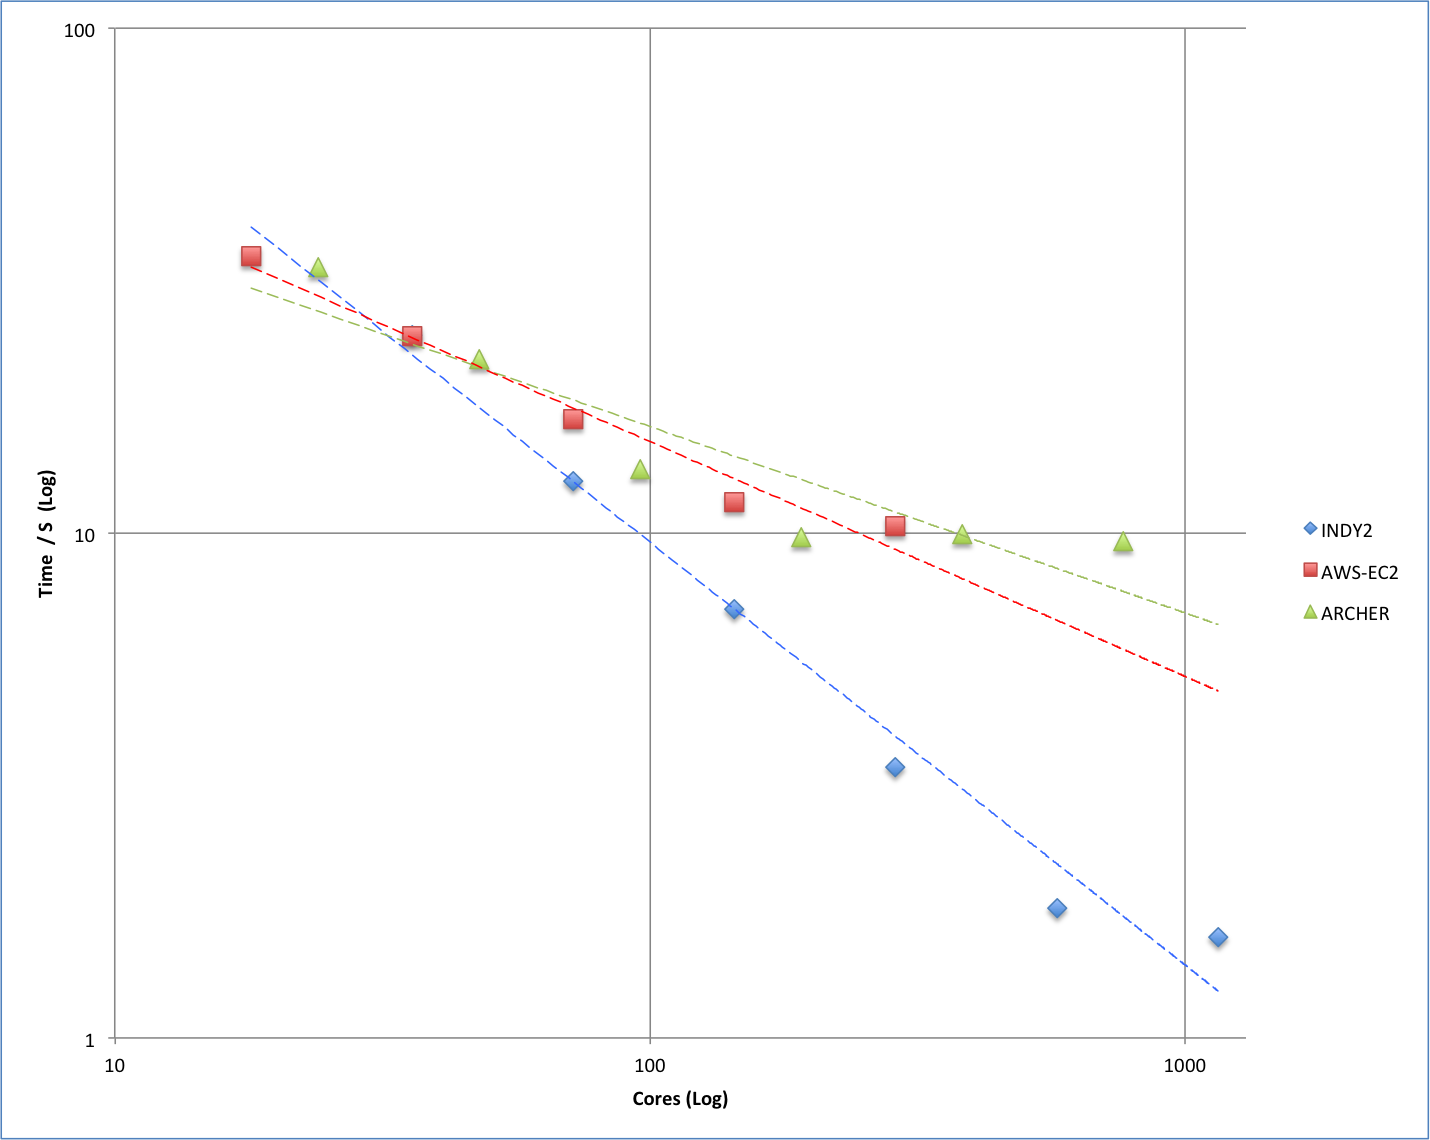
\includegraphics[keepaspectratio=true,scale=0.55]{../resources/evaluation/performance/overview.png}
 }
\captionof{figure}{HemeLB performance comparison} \label{fig:hemelb-perf-overview}%      only if needed  
\end{minipage}

\vspace{0.5cm}


Table \ref{table:perf} shows the performance comparison between HemeLB total simulation time at AWS-EC2 with INDY2. This shows that AWS-EC2 performance is much slower compared to the dedicated infrastructure likes INDY2. Table \ref{table:perf-archer} shows the HemeLB performance in ARCHER supercomputer. We cannot make a direct comparison between the performance of AWS-EC2 and INDY2 because ARCHER has a different number of cores in one compute node. ARCHER has 24, while AWS-EC2 and INDY2 have 36. Figure \ref{fig:hemelb-perf-overview} shows the performance difference and the scaling trend in a chart. 


For the simulation, we use an input file which has 4,520,681 fluid sites\footnote{Available online at \url{https://github.com/SeiryuZ/HemeWeb/blob/master/deployment/roles/hemeweb_master/files/990_Example2-skeleton_corrected_tubed_smoothed.gmy}}  \footnote{Config for the simulation can be found online at \url{https://github.com/SeiryuZ/HemeWeb/blob/master/documents/resources/evaluation/performance/config.xml}}. According to the performance analysis by Groen et al. \citep{groen2013analysing}, HemeLB scales up near-linearly up to 32,768 cores. It also performs near its maximum efficiency when using 5,000 to 500,000 sites per core. This means that for the problem size we use, HemeLB should perform near maximum efficiency when using 9 cores up to 900 cores. Above that core counts, HemeLB simulation will incur a performance penalty.

The simulation time of INDY2 as observed in Figure \ref{fig:hemelb-perf-overview} follows this performance model accurately. It scales almost linearly up to 576 cores, and finally hit a performance degradation on 1152 cores. However, the result on AWS-EC2 shows that HemeLB hits performance degradation much early that it does not follow the performance models. The reason being is that the infrastructure has an underlying difference in the networking capabilities. AWS-EC2 offer 10 Gigabit per second interface \footnote{\url{https://aws.amazon.com/premiumsupport/knowledge-center/network-throughput-benchmark-linux-ec2/}} while dedicated HPC infrastructure often uses InfiniBand or Cray Aries router interconnectivity which provides higher throughput \cite{Quan:2014aa}. This result is in line with the benchmark that Mehrotra et al. did on NASA's HPC application \citep{mehrotra2012performance}. The performance degradation comes from the network and the virtualization overhead that this cloud platform has.  ARCHER supercomputer in this benchmark, however, shows the performance that does not follow the performance model closely. As we increase the core number, the simulation time decrease, but not near linearly. In addition, there is some dip in performance at 384 cores. This erratic results might be due to the random nature of the workload on ARCHER. 

ARCHER supercomputer has slower simulation time compared to INDY2, because of the difference of processors used in the compute node. ARCHER used a three-year-old 2.7 GHz, 12-core E5-2697 v2 Ivy Bridge processor. Compared to INDY2 which boasts the newer Broadwell-based Intel Xeon CPU E5-2695 v4 @ 2.10GHz. The number of thread inside those processors also differ, ARCHER has 24 while INDY2 has 36. This makes the performance difference. On the other hand for this evaluation, we use Amazon's c4.8xlarge EC2 instance which has Haswell-based E5-2666 v3 processor that has 36 virtual CPU cores. All these difference contributes toward the speed difference of the simulation results.

The scaling of the performance is where HemeWeb took a dive. It is apparent that with increased compute node, the network activity between the nodes become a bottleneck in the HemeWeb's case. The performance started to dip when we use 4 compute nodes which have 144 cores which perform worse than just using 1 compute node. However, the performance improves as we add more compute nodes. Roughly speaking, HemeWeb run HemeLB simulation in AWS-EC2 1.46 times slower and up to 11.27 times slower at its worst when compared to the INDY2's performance. The performance difference is more apparent when INDY2 scale really well with larger cores, while in AWS-EC2, it didn't.

\subsection{Price performance analysis}

To analyze the performance even further, we can compare the performance we get with the price we have to pay to run the infrastructure. In running the simulation for benchmark, we used c4.8xlarge linux instances on EU Ireland region which at the time of writing costs GBP 1.51\footnote{USD 1.96 converted to GBP on https://\url{www.oanda.com/currency/converter/} at 13th August 2016} per hour\footnote{\url{https://aws.amazon.com/ec2/pricing/}}. Phase 2 XC30 ARCHER supercomputer give access to screened project by compute hour which has the price of GBP 0.56 for research council which are partnered and GBP 1.33 for  non-partnered research council\footnote{Calculated on \url{http://archer.ac.uk/access/au-calculator/}}. INDY2 however have no public pricing released by the EPCC yet.

With these pricing information, we can deduce that using AWS EC2 is 2.69 times more expensive compared to using ARCHER with partnership and 1.13 times more expensive without partnership. With more costs, using HemeWeb has lower performance but comparable to the ARCHER supercomputer. This cost is also compounded with the fact that job will finish much slower when using HemeWeb on AWS-EC2 infrastructure. It potentially run 2.69 times more expensive per hour but 11.27 (CHANGE THIS WHEN NEW DATA ARRIVE) times much slower compared to using dedicated HPC infrastructure like ARCHER. If a job finish in 1 hour in INDY2, it can run for almost 12 hours (CHANGE THIS WHEN NEW DATA ARRIVE) on ARCHER at its worst, which will cost much more. However, because there are no price information yet on INDY2, we cannot make any price performance comparison between AWS-EC2 with INDY2 that has bigger performance gap. 


All of this performance pricing analysis however have to take into account of the model of business of the governing institution. On using Amazon's resources, one does not have to submit a proposal or go to a resource allocation community, he / she just need a credit cards and access will be given. In addition to that, Amazon employ the pay-as-you-go pricing scheme so it is very flexible in changing requirements or usage compared to ARCHER which allocate the resources at the start of the project. 


\section {Limitation of the evaluations}

\subsection{Usability evaluation}

When observing the evaluation, one might argue that 5 point scale used in the questionnaire is not enough as pointed out by Kraig Finstad \cite{finstad2010response}. In his research, he argued that 5 point scale for a questionnaire allows more room for respondents to interpolate their response. He compared the same version of usability study but with five-point and seven-point scale and found out that 3\% of the respondents answer to five point scale actually are interpolation, while the seven point scale have no interpolation. He concluded that administering usability study using seven point scale will achieve greater accuracy. However, I decided to use the five point scale of the questionnaire because of the limitation of google survey platform. 

\noindent%
\begin{minipage}{\linewidth}% to keep image and caption on one page
\makebox[\linewidth]{
  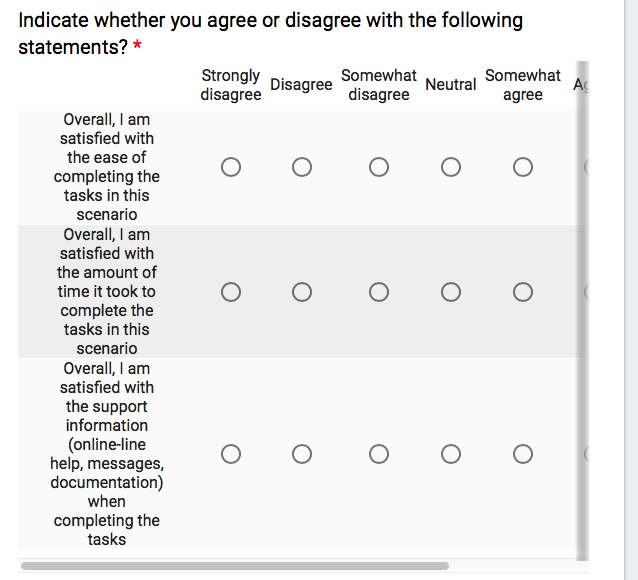
\includegraphics[keepaspectratio=true,scale=0.35]{../resources/images/google-limitation.png}
 }
\captionof{figure}{Google form hiding some options on 7 point scale} \label{fig:google-limit}%      only if needed  
\end{minipage}


\vspace{0.5cm}
\noindent%
\begin{minipage}{\linewidth}% to keep image and caption on one page
\makebox[\linewidth]{
  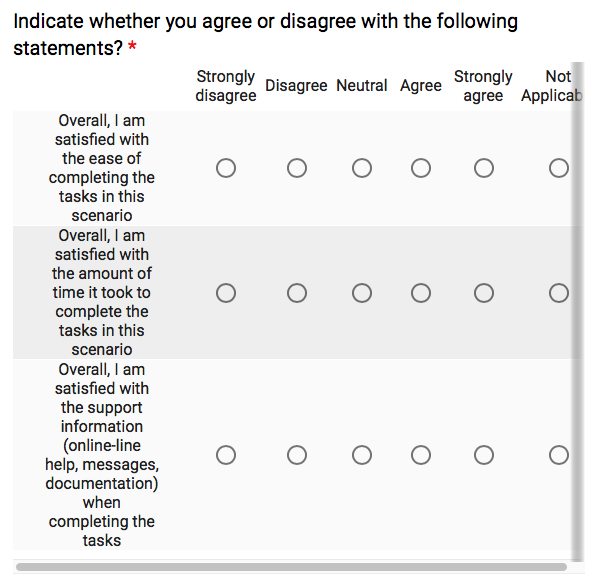
\includegraphics[keepaspectratio=true,scale=0.35]{../resources/images/google-limitation2.png}
 }
\captionof{figure}{Google form render 5 point scale rating better} \label{fig:google-limit2}%      only if needed  
\end{minipage}

\vspace{0.5cm}


Figure \ref{fig:google-limit} show the limitation of the platform. The response options are not rendered in complete, as in some are hidden in a scrolling element of the page. This leads to respondents have to scroll left and right to see the options and answers. I find this is a detriment to the respondents to do more work in answering the question so I decided to use 5 point scale to make sure everything is rendered better like shown in Figure \ref{fig:google-limit2}.


Another limitation of the study is the way the study compare the experience of doing the scenarios in the questionnaire between using web browser and using command line.  When measuring the usability of HemeWeb, respondents are asked to do the task in the web browser, compared to the task in command line where it is just described in an overview. This decision is made because we cannot make sure the respondents have the necessary tools to run or reproduce a simulation in their computers.  In addition, in order to run the scenario in command line interface, respondents have to install tools on their computer which are timely and prone to errors. I believe this will affect their sentiment in answering the survey questionnaire and decided against it.


\subsection{Performance evaluation}

On running the HemeLB simulation on the three systems compared, we cannot fully isolate the infrastructure from various system load the infrastructure is handling. The performance might be affected by other jobs running in the system, which is apparent in the case of ARCHER supercomputer where many jobs are executing at the same moment. The same case with INDY2. The performance benchmark might be not as accurate as a completely isolated environment, however it paints a pretty good picture of performance you get when using cloud vendors compared to the dedicated infrastructure. 

Also another limitation on the performance evaluation is that we cannot get more than 20 instances of c4.8xlarge instances on AWS. This causes the evaluation for AWS-EC2 cannot be done for the 1,152 cores to compare it directly with INDY2. Another limitation is that on ARCHER, it has 24 cores in 1 compute node compared to 36 in INDY2 and AWS-EC2. We wanted to measure the full load of the compute node, therefore we cannot get an exact apple to apple comparison. However, it could help in painting the general trend of the scaling capabilities and measure based on that.
 
